% Created by tikzDevice version 0.8.1 on 2015-05-24 13:12:07
% !TEX encoding = UTF-8 Unicode
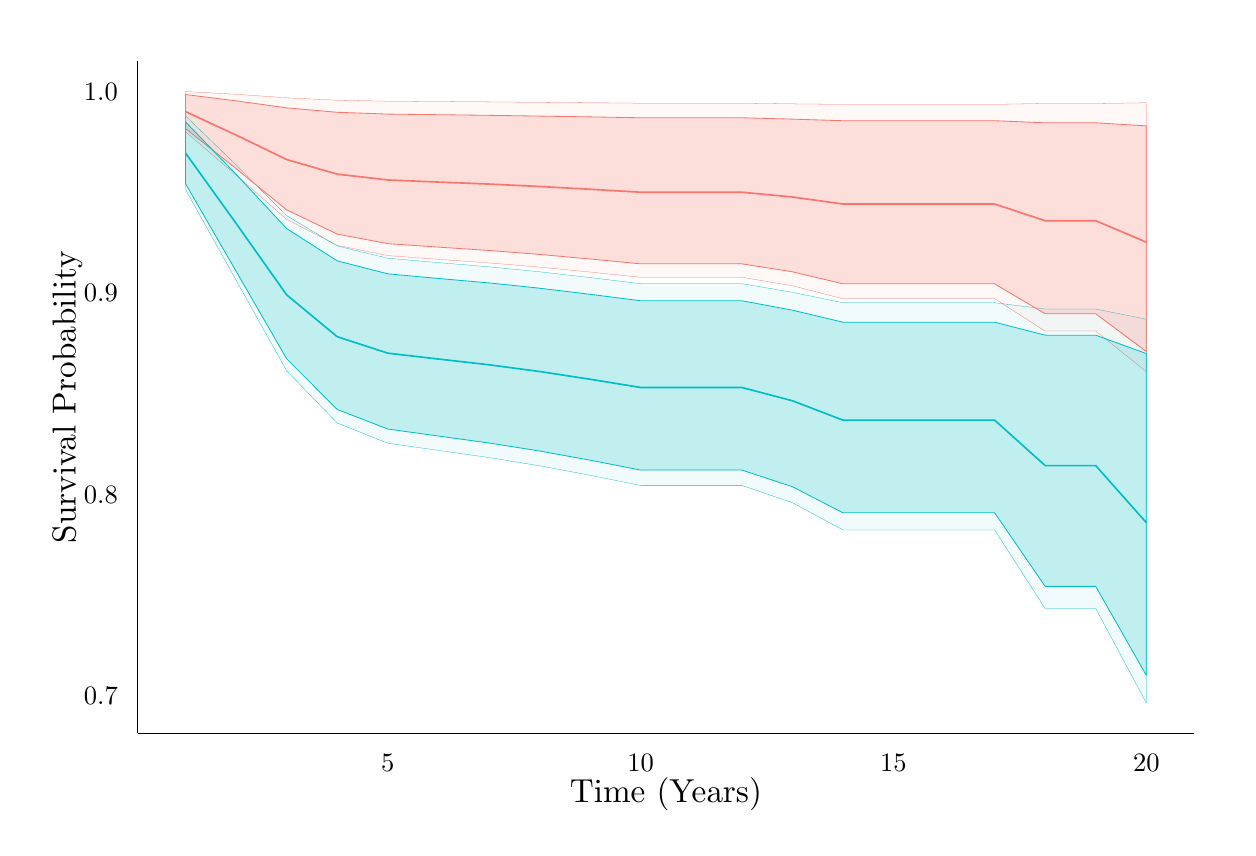
\begin{tikzpicture}[x=1pt,y=1pt]
\definecolor{fillColor}{RGB}{255,255,255}
\path[use as bounding box,fill=fillColor,fill opacity=0.00] (0,0) rectangle (433.62,289.08);
\begin{scope}
\path[clip] (  0.00,  0.00) rectangle (433.62,289.08);
\definecolor{drawColor}{RGB}{255,255,255}
\definecolor{fillColor}{RGB}{255,255,255}

\path[draw=drawColor,line width= 0.6pt,line join=round,line cap=round,fill=fillColor] (  0.00,  0.00) rectangle (433.62,289.08);
\end{scope}
\begin{scope}
\path[clip] ( 39.69, 34.03) rectangle (421.57,277.03);
\definecolor{fillColor}{RGB}{255,255,255}

\path[fill=fillColor] ( 39.69, 34.03) rectangle (421.58,277.03);
\definecolor{drawColor}{RGB}{248,118,109}

\path[draw=drawColor,line width= 0.6pt,line join=round] ( 57.05,258.74) --
	( 75.32,250.27) --
	( 93.59,241.43) --
	(111.86,236.15) --
	(130.13,234.05) --
	(148.41,233.29) --
	(166.68,232.56) --
	(184.95,231.69) --
	(203.22,230.69) --
	(221.49,229.62) --
	(239.77,229.62) --
	(258.04,229.62) --
	(276.31,227.90) --
	(294.58,225.35) --
	(312.86,225.35) --
	(331.13,225.35) --
	(349.40,225.35) --
	(367.67,219.32) --
	(385.94,219.32) --
	(404.22,211.58);
\definecolor{drawColor}{RGB}{0,191,196}

\path[draw=drawColor,line width= 0.6pt,line join=round] ( 57.05,243.76) --
	( 75.32,218.35) --
	( 93.59,192.52) --
	(111.86,177.41) --
	(130.13,171.46) --
	(148.41,169.34) --
	(166.68,167.26) --
	(184.95,164.84) --
	(203.22,162.04) --
	(221.49,159.07) --
	(239.77,159.07) --
	(258.04,159.07) --
	(276.31,154.27) --
	(294.58,147.26) --
	(312.86,147.26) --
	(331.13,147.26) --
	(349.40,147.26) --
	(367.67,130.84) --
	(385.94,130.84) --
	(404.22,110.22);
\definecolor{drawColor}{RGB}{248,118,109}
\definecolor{fillColor}{RGB}{248,118,109}

\path[draw=drawColor,line width= 0.1pt,line join=round,line cap=round,fill=fillColor,fill opacity=0.05] ( 57.05,265.99) --
	( 75.32,265.02) --
	( 93.59,263.74) --
	(111.86,262.86) --
	(130.13,262.51) --
	(148.41,262.39) --
	(166.68,262.26) --
	(184.95,262.11) --
	(203.22,261.96) --
	(221.49,261.79) --
	(239.77,261.79) --
	(258.04,261.79) --
	(276.31,261.55) --
	(294.58,261.37) --
	(312.86,261.37) --
	(331.13,261.37) --
	(349.40,261.37) --
	(367.67,261.68) --
	(385.94,261.68) --
	(404.22,261.93) --
	(404.22,164.75) --
	(385.94,179.44) --
	(367.67,179.44) --
	(349.40,191.13) --
	(331.13,191.13) --
	(312.86,191.13) --
	(294.58,191.13) --
	(276.31,195.81) --
	(258.04,198.89) --
	(239.77,198.89) --
	(221.49,198.89) --
	(203.22,200.77) --
	(184.95,202.55) --
	(166.68,204.07) --
	(148.41,205.37) --
	(130.13,206.71) --
	(111.86,210.42) --
	( 93.59,219.80) --
	( 75.32,235.81) --
	( 57.05,251.44) --
	cycle;
\definecolor{drawColor}{RGB}{0,191,196}
\definecolor{fillColor}{RGB}{0,191,196}

\path[draw=drawColor,line width= 0.1pt,line join=round,line cap=round,fill=fillColor,fill opacity=0.05] ( 57.05,257.18) --
	( 75.32,239.53) --
	( 93.59,221.15) --
	(111.86,210.20) --
	(130.13,205.77) --
	(148.41,204.18) --
	(166.68,202.68) --
	(184.95,200.86) --
	(203.22,198.78) --
	(221.49,196.58) --
	(239.77,196.58) --
	(258.04,196.58) --
	(276.31,193.47) --
	(294.58,189.68) --
	(312.86,189.68) --
	(331.13,189.68) --
	(349.40,189.68) --
	(367.67,187.41) --
	(385.94,187.41) --
	(404.22,183.74) --
	(404.22, 45.08) --
	(385.94, 79.19) --
	(367.67, 79.19) --
	(349.40,107.60) --
	(331.13,107.60) --
	(312.86,107.60) --
	(294.58,107.60) --
	(276.31,117.43) --
	(258.04,123.69) --
	(239.77,123.69) --
	(221.49,123.69) --
	(203.22,127.34) --
	(184.95,130.77) --
	(166.68,133.74) --
	(148.41,136.33) --
	(130.13,138.92) --
	(111.86,146.22) --
	( 93.59,165.09) --
	( 75.32,197.80) --
	( 57.05,230.58) --
	cycle;
\definecolor{drawColor}{RGB}{248,118,109}
\definecolor{fillColor}{RGB}{248,118,109}

\path[draw=drawColor,line width= 0.3pt,line join=round,line cap=round,fill=fillColor,fill opacity=0.20] ( 57.05,264.92) --
	( 75.32,262.63) --
	( 93.59,260.11) --
	(111.86,258.50) --
	(130.13,257.85) --
	(148.41,257.63) --
	(166.68,257.40) --
	(184.95,257.13) --
	(203.22,256.84) --
	(221.49,256.52) --
	(239.77,256.52) --
	(258.04,256.52) --
	(276.31,256.03) --
	(294.58,255.45) --
	(312.86,255.45) --
	(331.13,255.45) --
	(349.40,255.45) --
	(367.67,254.70) --
	(385.94,254.70) --
	(404.22,253.59) --
	(404.22,172.05) --
	(385.94,185.69) --
	(367.67,185.69) --
	(349.40,196.52) --
	(331.13,196.52) --
	(312.86,196.52) --
	(294.58,196.52) --
	(276.31,200.87) --
	(258.04,203.74) --
	(239.77,203.74) --
	(221.49,203.74) --
	(203.22,205.49) --
	(184.95,207.15) --
	(166.68,208.57) --
	(148.41,209.78) --
	(130.13,211.03) --
	(111.86,214.50) --
	( 93.59,223.23) --
	( 75.32,238.12) --
	( 57.05,252.61) --
	cycle;
\definecolor{drawColor}{RGB}{0,191,196}
\definecolor{fillColor}{RGB}{0,191,196}

\path[draw=drawColor,line width= 0.3pt,line join=round,line cap=round,fill=fillColor,fill opacity=0.20] ( 57.05,255.00) --
	( 75.32,236.08) --
	( 93.59,216.47) --
	(111.86,204.82) --
	(130.13,200.13) --
	(148.41,198.45) --
	(166.68,196.85) --
	(184.95,194.94) --
	(203.22,192.73) --
	(221.49,190.40) --
	(239.77,190.40) --
	(258.04,190.40) --
	(276.31,187.00) --
	(294.58,182.66) --
	(312.86,182.66) --
	(331.13,182.66) --
	(349.40,182.66) --
	(367.67,177.96) --
	(385.94,177.96) --
	(404.22,171.31) --
	(404.22, 55.03) --
	(385.94, 87.18) --
	(367.67, 87.18) --
	(349.40,113.79) --
	(331.13,113.79) --
	(312.86,113.79) --
	(294.58,113.79) --
	(276.31,123.20) --
	(258.04,129.24) --
	(239.77,129.24) --
	(221.49,129.24) --
	(203.22,132.79) --
	(184.95,136.12) --
	(166.68,139.01) --
	(148.41,141.52) --
	(130.13,144.04) --
	(111.86,151.13) --
	( 93.59,169.42) --
	( 75.32,201.06) --
	( 57.05,232.68) --
	cycle;
\end{scope}
\begin{scope}
\path[clip] (  0.00,  0.00) rectangle (433.62,289.08);
\definecolor{drawColor}{RGB}{0,0,0}

\path[draw=drawColor,line width= 0.6pt,line join=round] ( 39.69, 34.03) --
	( 39.69,277.03);
\end{scope}
\begin{scope}
\path[clip] (  0.00,  0.00) rectangle (433.62,289.08);
\definecolor{drawColor}{RGB}{0,0,0}

\node[text=drawColor,anchor=base east,inner sep=0pt, outer sep=0pt, scale=  0.96] at ( 32.57, 44.50) {0.7};

\node[text=drawColor,anchor=base east,inner sep=0pt, outer sep=0pt, scale=  0.96] at ( 32.57,117.23) {0.8};

\node[text=drawColor,anchor=base east,inner sep=0pt, outer sep=0pt, scale=  0.96] at ( 32.57,189.96) {0.9};

\node[text=drawColor,anchor=base east,inner sep=0pt, outer sep=0pt, scale=  0.96] at ( 32.57,262.68) {1.0};
\end{scope}
\begin{scope}
\path[clip] (  0.00,  0.00) rectangle (433.62,289.08);
\definecolor{drawColor}{RGB}{0,0,0}

\path[draw=drawColor,line width= 0.6pt,line join=round] ( 39.69, 34.03) --
	(421.57, 34.03);
\end{scope}
\begin{scope}
\path[clip] (  0.00,  0.00) rectangle (433.62,289.08);
\definecolor{drawColor}{RGB}{0,0,0}

\node[text=drawColor,anchor=base,inner sep=0pt, outer sep=0pt, scale=  0.96] at (130.13, 20.31) {5};

\node[text=drawColor,anchor=base,inner sep=0pt, outer sep=0pt, scale=  0.96] at (221.49, 20.31) {10};

\node[text=drawColor,anchor=base,inner sep=0pt, outer sep=0pt, scale=  0.96] at (312.86, 20.31) {15};

\node[text=drawColor,anchor=base,inner sep=0pt, outer sep=0pt, scale=  0.96] at (404.22, 20.31) {20};
\end{scope}
\begin{scope}
\path[clip] (  0.00,  0.00) rectangle (433.62,289.08);
\definecolor{drawColor}{RGB}{0,0,0}

\node[text=drawColor,anchor=base,inner sep=0pt, outer sep=0pt, scale=  1.20] at (230.63,  9.03) {Time (Years)};
\end{scope}
\begin{scope}
\path[clip] (  0.00,  0.00) rectangle (433.62,289.08);
\definecolor{drawColor}{RGB}{0,0,0}

\node[text=drawColor,rotate= 90.00,anchor=base,inner sep=0pt, outer sep=0pt, scale=  1.20] at ( 17.30,155.53) {Survival Probability};
\end{scope}
\end{tikzpicture}
